\documentclass[11pt]{article}
\usepackage{fullpage}

\title{Natural User Interface and Virtual Reality Integration\\in Video Games\\{\small Last Revised: \today}}
\author{\small\begin{tabular}{c c c c} 
		Alexandre Wimmers 		& Mario Yepez 			& Timothy Tong			& Valerie Gadjali\\
		adwimmers@ucdavis.edu 	& myepez@ucdavis.edu 	& tktong@ucdavis.edu	& vgadjali@ucdavis.edu
	\end{tabular}}
\date{}

\usepackage{graphicx}
\usepackage{float}
\usepackage{array} 

\begin{document}

\maketitle

\section{Background}

\subsection{Natural User Interface}

\paragraph{} Natural user interface is the ability to use an application without the need for any controller. In this case, the players own body or parts of the body becomes the controller. The concept of natural user interface first appeared in 1990, but the first popular usage for video games appeared in 2010 with the release of the Microsoft Kinect. Traditional keyboards and mice can only interact with a monitor or any visual interface in a two-dimensional sense. However, with a natural user interface it becomes possible to interact in three dimensions.

\subsection{Virtual Reality}

\paragraph{} Virtual reality is an immersive experience within a computer-simulated environment. First conceptualized in 1930, but only recently has it become a popular with the Oculus Rift Development Kit 1. It provides the user a complete immersion and a new perspective into the virtual world. Whereas a monitor restricts a user to only view in two dimensions, virtual reality allows the user to see the world in three dimensions.

\subsection{Unity Game Engine}

\paragraph{} Unity is the game engine of choice for this project. Developed by Unity Technologies, Unity includes both a game engine and an integrated development environment. There are a variety of factors that led to the adoption of Unity, such as portability. Games built on Unity are able to run on multiple platforms; this allows for game development regardless of operating system. A host of plug-ins and libraries are also available for Unity such as the A* Pathfinding Project and Photon, which will prove to be useful in development of this project. The most notable plug-in and library is the Oculus Rift and Leap Motion compatibility. Other game engines require workarounds while Unity makes integration simple. 

\section{Goal}

\paragraph{} Take an existing video game genre and develop a video game integrating both natural user interface and virtual reality.

\section{Game Genres}

\subsection{Real-Time Strategy (RTS)}

\paragraph{} As a subcategory of strategy video games, real-time strategy is a type of war game that requires you to manage resources and fight with an opponent in real time. Unlike turn-based games, RTS games require quick reaction and thinking to succeed. The term real-time strategy first appeared in 1982 in a game called Cytron Masters by Dani Bunten Berry. 

\subsubsection{Pros}

\begin{itemize}
	\item True three dimensional real-time strategy.
	\item "Cool" factor for in-person perspective with combat.
	\item High customization.
\end{itemize}

\subsubsection{Cons}

\begin{itemize}
	\item Steep learning curve.
	\item Reduced precision in controls due to technology.
	\item In-person perspective has no objective gain in competitive gameplay, but rather impedes player. Zooming out to bird's eye view while aligning to one of three axis will provide a much more effective perspective which defeats the purpose of certain technologies in this game.
\end{itemize}

\subsection{Castle Defense}

\paragraph{} The original version of Castle Defense was a Flash-based browser video game called ``Defend Your Castle". In this game, there were a series of different enemies who would walk to the castle and attack it, but all of them were in a stick figure art style. Players were to prevent enemies from destroying the castle, by using a variety of methods, such as drag and dropping the enemies or flinging them away. In 2008, a milder version of this game was released on the Wii and included a multiplayer mode. The weapons that were used were daily household items and the use of blood was removed. In 2009, an iOS version was release and implemented the finger-touch method for controls rather than a mouse. This game genre has received completely mixed reviews; some critics and users enjoyed the game play, but disliked the graphics, while many thought the vice versa.

\subsubsection{Pros}

\begin{itemize}
	\item Easy to pickup and play.
	\item Requires less precision for hand gestures.
\end{itemize}

\subsubsection{Cons}

\begin{itemize}
	\item Near zero gameplay customization.
	\item Standard gameplay is simpler in complexity compared to real-time strategy.
\end{itemize}

\section{Implementation}

\subsection{Genre of Choice}

\paragraph{} Castle Defense.

\paragraph{} After weighing the Pros and Cons of both game genres the team opted for the Castle Defense game. Castle Defense targets a wider audience of players and this is mainly due to the fact that there is a steeper learning curve for a Real Time Strategy game. Another critical reason was the fact that, for the real-time strategy game, the standard birds-eye view was more effective than the virtual reality in-person view. People of all ages will be able to pick up and play the game easily and start having fun.

\subsection{Game Flow}

\begin{figure}[H]
	\centering
	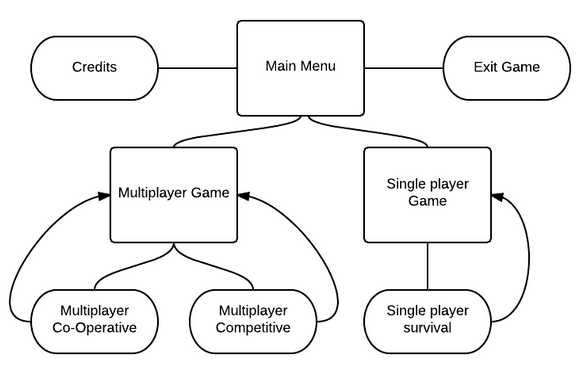
\includegraphics{../images/castle-defense-game-flow.png}
\end{figure}

\paragraph{} One of the core principles for designing the game was to allow the user to jump right into the action and start playing without the hassle of navigating through a series of menus. Menus break immersion if done incorrectly, which is why we have decided to minimize menus as much as possible. As can be seen from the flow-chart above, the user does not need to fiddle with options to get into the game. 

\subsection{Victory Conditions}

\paragraph{} Victory conditions will vary depending on the type of game mode that the player(s) select. 

\paragraph{} For the Single Player Survival and Multiplayer Cooperative mode, the user(s) must survive wave after wave of enemies that attack their castle. If the player(s) manage(s) to defend the castle against a set number of waves then they will win the game and be sent to a “Victory!” screen. However if the player fails to do so they will be sent to a ``Game Over!" screen.

\paragraph{} For the Multiplayer Competitive mode, two players will compete with each other to see who is the dominant one. Player A will be be defending the castle as in the Single Player Survival mode. Player B will take control of the waves that are attacking the castle. Player B will be responsible for spawning the waves and sending them through paths that lead to the castle. If Player A successfully fends off 3 waves Player A will be declared the victor. On the other hand, if Player A fails to do so then Player B will win the game.

\subsection{Enemy Hierarchy}

\subsubsection{Basic Stickman}

\begin{figure}[H]
	\centering
	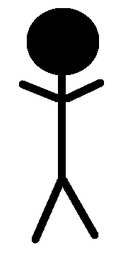
\includegraphics{../images/castle-defense-basic-stickman.png}
\end{figure}

\paragraph{} This is the first enemy that players will encounter. They are the weakest of two that will be introduced in Prototype I. They will not be too difficult to dispose of and serve more as a tutorial for players who are first coming into the game.

\begin{table}[H]
	\centering
	\begin{tabular}{c >{\(}c<{\)}}
		Health Rating	&	\star \star \star\\
		Attack Rating	&	\star \star \star\\
		Defense Rating	&	\star\\
		Speed Rating	&	\star \star \star
	\end{tabular}
\end{table}

\subsubsection{Bulky Stickman}

\begin{figure}[H]
	\centering
	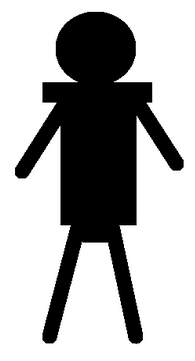
\includegraphics{../images/castle-defense-bulky-stickman.png}
\end{figure}

\paragraph{} After fending off Basic Stickman the player will now encounter a new foe, the mighty Bulky Stickman. The Bulky Stickman is stronger than Basic Stickman, but it comes at a cost. The armor weighs down the Stickman and slows him down.

\begin{table}[H]
	\centering
	\begin{tabular}{c >{\(}c<{\)}}
		Health Rating	&	\star \star \star \star \star\\
		Attack Rating	&	\star \star \star \star \star\\
		Defense Rating	&	\star \star \star\\
		Speed Rating	&	\star
	\end{tabular}
\end{table}

\subsection{Technology Integration}

\subsubsection{Natural User Interface}

The traditional castle defense utilized a mouse to drag and drop stickmen. Through dropping the stickmen at elevated heights and effects of gravity, the enemy stickmen are defeated. With the use of natural user interface, the player will use his or her hands in place of the mouse. The natural user interface device will capture the player's hands motions in the physical realm and virtualize them in the digital world. When the player's hands closes around a stickmen, it will effectively grab the stickmen for dragging. 

\subsubsection{Virtual Reality}

Bounded by only the use of a monitor, the classic perspective in castle defense in from a sideways angle where the castle resides on one end of the map and stickmen spawn from the other end. By making the game three-dimensional, the map becomes a three-dimensional plane with the castle residing in the center and the stickmen spawn on the outskirts of the plane. Naturally with three-dimensions, it utilizes a virtual camera that creates the perspective similarly to games like first-person shooters. The virtual reality device can therefore simply synchronize with this virtual camera. 


\end{document}